\chapter{Fundamentação Teórica}
\label{chap:fund}

Neste capítulo serão abordados os principais conceitos de \emph{Deep Learning}, assim como as técnicas e algoritmos aplicados para auxiliar os profissionais de laboratório a realizarem exames de sangue de uma forma automatizada e eficiente. Além disso, será detalhado sobre os hemogramas e diferentes dados coletados através de uma análise de sangue.

\section{Exames Laboratoriais de Sangue}
\label{sec:conceito1}
Os exames laboratoriais de sangue, principalmente se tratando de hemogramas, são um tipo de exame simples porém de extrema importância para a saúde humana. Através desses exames pode-se descobrir diversas informações sobre o organismo da pessoa em questão, inclusive detectar doenças e problemas de forma antecipada, como por exemplo para diagnosticar anemia, deficiências nutricionais, parasitas no sangue, doenças virais e autoimunes. Também é possível identificar infecções, doenças como leucemia, diagnosticar efeitos de medicamentos e também o efeito de vários tipos de estresse sobre o corpo \cite{abcOfCbc, atlasDeHematologiaEAnalise}.

Um exame poderá ser solicitado por um médico, ou a partir do interesse do próprio paciente, e realizado em um laboratório de confiança, que será responsável por realizar a coleta, encaminhar para a análise específica e retornar o resultado. Todo esse processo é custoso em tempo de espera e também financeiramente, pois o maquinário para esse tipo de atividade é muito caro para aquisição e manutenção.

\subsection{Sangue}
O sangue é um elemento do corpo humano, que circula em estado líquido através de todo o sistema circulatório do organismo, sendo de importância para o funcionamento correto das células através da entrada e saída de substâncias que podem modificar a sua composição \cite{manualHematologia}.

Pode ser dividido em duas principais partes: o plasma (ou soro) e a parte celular. O plasma é a principal parte de transporte de substâncias pelo sistema, sendo este formado pela ingestão de água e alimentos. Também pode ser chamado de soro, sendo possível diferenciá-los pela presença ou não de anticoagulantes utilizados dependendo do tipo da análise buscada e da intenção da pesquisa \cite{manualHematologia}.

A segunda parte do sangue, que será objeto de estudo para este trabalho, é a parte celular que contém todas as células presentes no sangue e se classificam como glóbulos vermelhos, glóbulos brancos e plaquetas. Geralmente observa-se a presença de eritrócitos, vários tipos e classes de leucócitos e as plaquetas como um todo, que serão abordados um a um posteriormente \cite{manualHematologia}.

\subsubsection{Glóbulos Vermelhos}
Os glóbulos vermelhos, também conhecidos como \emph{Red Blood Cells (RBC)}, são as hemácias presentes no sangue, também podem ser citadas em exames e registros médicos como eritrócitos. Essas células são pequenas e circulares, geralmente em formatos de discos e não possuem núcleo. Estão presentes em grande quantidade, possuindo uma vida útil de aproximadamente 120 dias até que o próprio sistema as elimine \cite{manualHematologia}.

É indispensável ao falar sobre a parte vermelha do sangue, citar a hemoglobina que é uma proteína presente nas hemácias e de extrema importância para o funcionamento do sistema, pois através dela é possível realizar o transporte de oxigênio e gás carbônico pelo sistema sanguíneo, permitindo as trocas gasosas necessárias \cite{manualHematologia}.

Podemos perceber a presença dos glóbulos vermelhos na imagem \ref{fig:rbc}, onde estão em grande quantidade em comparação com as outras células. 

\begin{figure}[!htb]
	\centering
	\caption{Glóbulos Vermelhos (RBC)}
	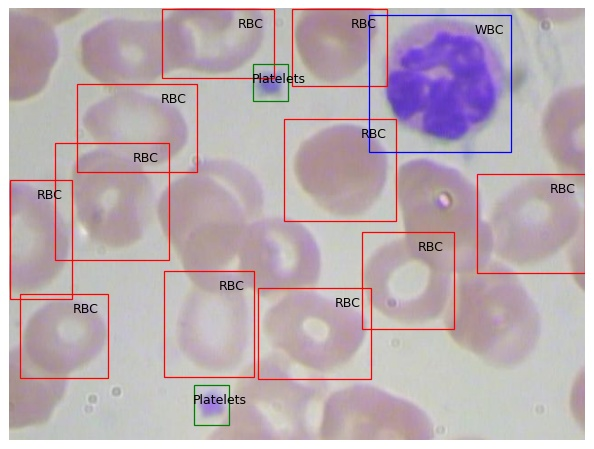
\includegraphics[width=0.40\textwidth]{img/rbc.jpg}
	\legend{Fonte: \cite{datasetBCCD}}
	\label{fig:rbc}
\end{figure}

A imagem \ref{fig:rbc} foi retirada de um \emph{dataset} específico de classificação de células sanguíneas, classificando em RBC (Red Blood Cells) para glóbulos vermelhos, WBC (White Blood Cells) para glóbulos brancos e Platelets para plaquetas.
 
\subsubsection{Glóbulos Brancos}
Os glóbulos brancos, também conhecidos como \emph{White Blood Cells (WBC)}, são as células brancas do sangue, sendo responsáveis pela defesa do organismo contra as principais ameaças do corpo humano presentes no sistema sanguíneo. Através da fagocitose, que é um processo de englobamento de partículas sólidas pelas células, são realizadas ações de defesa contra a invasão de fragmentos estranhos. Os glóbulos brancos são criados na medula óssea e estão presentes em todo o sangue, também em grande quantidade \cite{manualHematologia}.

Se faz necessário a classificação dos diferentes tipos de células brancas e de suas importâncias para o sistema de defesa do organismo. É importante frisar que essa classificação se refere aos leucócitos maduros, mas também pode-se encontrar presente os leucócitos imaturos (promielócitos, mielócitos, metamielócitos) \cite{manualHematologia}.

\begin{itemize}
	\item \textbf{Neutrófilos}: células brancas mais abundantes capazes de entrar nos tecidos, onde conseguem realizar a defesa do organismo, fagocitando partículas estranhas. Essas células são conhecidas como neutrófilos segmentados, pois existe uma célula percursora, que é o bastão, ou também chamado de neutrófilos bastonetes, que possuem essa nomenclatura pois seu núcleo não está amadurecido, ou seja ainda são jovens, e geralmente são identificados quando há infecções em fase aguda. 
	\item \textbf{Eosinófilos}: células brancas responsáveis na defesa contra parasitas, geralmente estão presentes em grande quantidade no sangue durante reações alérgicas e infestações parasitárias.
	\item \textbf{Basófilos}: células brancas atuantes em respostas alérgicas e na coagulação do sangue. São capazes de liberar histamina, contribuindo para respostas alérgicas ao dilatar e permeabilizar os vasos sanguíneos e também liberam heparina que é capaz de prevenir a coagulação do sangue.
	\item \textbf{Monócitos}: células brancas capazes de entrar no tecido conjuntivo frouxo, onde conseguem se desenvolver em grandes células com grande efeito fagocítico denominadas macrófagos, de forma a ingerir partículas estranhas ao organismo.
	\item \textbf{Linfócitos}: segundo tipo de célula branca mais abundante, são responsáveis e de extrema importância nas respostas imunes específicas do corpo humano, inclusive na produção de anticorpos.
\end{itemize}

Podemos perceber também na imagem \ref{fig:wbc} a presença dos glóbulos brancos entre os vermelhos.

\begin{figure}[!htb]
	\centering
	\caption{Glóbulos Brancos (WBC)}
	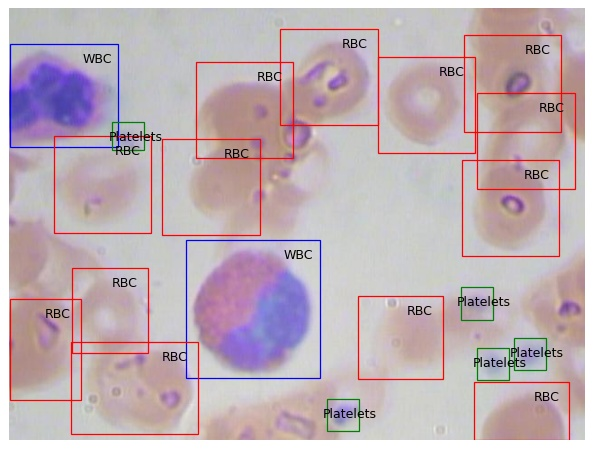
\includegraphics[width=0.40\textwidth]{img/wbc.jpg}
	\legend{Fonte: \cite{datasetBCCD}}
	\label{fig:wbc}
\end{figure}

Com visto na imagem \ref{fig:wbc}, embora existam várias classificações de glóbulos brancos, no \emph{dataset} onde a imagem foi coletada não era objetivo de estudo realizar essa análise específica de cada célula.

\subsubsection{Plaquetas}
As plaquetas, também conhecidas e citadas como \emph{Platelets}, são os menores componentes do sangue e possuem grande responsabilidade na hemostasia, que é uma resposta fisiológica para a prevenção e interrupção de sangramentos e hemorragias, ou seja, elas atuam na manutenção dos vasos sanguíneos. As plaquetas são fragmentos do citoplasma de megacariócitos, ou seja, elas são produzidas na medula óssea como parte dessas células especializadas que irão se dividir posteriormente e gerar um grande número de plaquetas. Aproximadamente, para cada 1 megacariócito, pode-se produzir cerca de 4000 plaquetas \cite{abcOfCbc}.

Devido ao fato de serem fragmentos de uma célula, as plaquetas não possuem núcleo e são muito pequenas, com aproximadamente de 1–3 µm de diâmetro, com a coloração azul-acinzentado. A vida útil das plaquetas dura em média de 9 a 12 dias, e elas são removidas pelo baço quando estão velhas ou danificadas \cite{abcOfCbc}.

Podemos perceber também através da imagem \ref{fig:plaquetas}, a presença do último elemento visível abordado por este trabalho no \emph{dataset} utilizado como base. Onde é possível visualizar múltiplas plaquetas agrupadas em um dos cantos da imagem, além de outras no meio dos demais elementos do sangue.

\begin{figure}[!htb]
	\centering
	\caption{Plaquetas (Platelets)}
	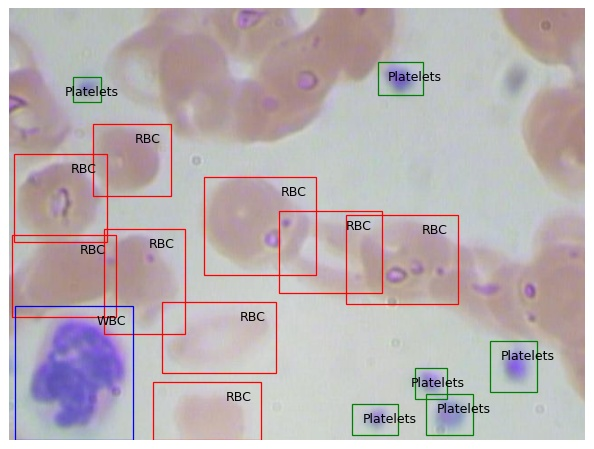
\includegraphics[width=0.40\textwidth]{img/plt.jpg}
	\legend{Fonte: \cite{datasetBCCD}}
	\label{fig:plaquetas}
\end{figure}

\subsection{Hemograma}
Um hemograma, também conhecido e citado como \emph{Complete Blood Count (CBC)}, é um exame bastante comum e muito utilizado, onde se realiza uma análise de sangue que envolve a contagem das diferentes células sanguíneas. A partir dos números obtidos através dessa contagem e com a comparação desse valor com as faixas de normalidade, é possível chegar a diversas conclusões sobre a saúde do paciente e até mesmo já identificar alguma doença ou problema \cite{manualHematologia, abcOfCbc}.

Um hemograma geralmente é realizado em duas principais etapas, sendo a primeira relacionada ao eritrograma que se refere à análise das células vermelhas, de forma a revelar até mesmo alguns tipos essenciais de alterações patológicas do sistema eritropoético, que é o sistema responsável pela produção do material vermelho do sangue, como aumento na produção de glóbulos vermelhos e anemias. A segunda parte está relacionada com o leucograma, que corresponde à contagem global e específica dos leucócitos, a parte branca do sangue. O quadro leucocitário resultante com o exame hematológico, possibilita ao médico tirar importantes conclusões \cite{manualHematologia, abcOfCbc}.

\subsubsection{Eritrograma}
O objetivo do eritrograma ao realizar a análise da parte vermelha do sangue, é analisar alguns atributos chave. Primeiramente é realizado a contagem geral dos eritrócitos adotando uma escala de milhões/mm³. A hemoglobina também será calculada e registrada em uma escala de g/dl \cite{interpretacaoHemograma, manualHematologia}.

Depois dessa principal contagem são calculados alguns índices importantes, sendo o primeiro deles o cálculo do volume corpuscular médio (VCM), que é o volume médio das hemácias, calculado pelo quociente de um determinado volume de hemácias pelo número de células contidas no mesmo volume. Outro importante atributo é a hemoglobina corpuscular média (HCM), que semelhante ao VCM, é o conteúdo médio da hemoglobina, calculado pelo quociente de conteúdo de hemoglobina em um determinado volume de hemácias pelo número de células contidas no mesmo volume \cite{interpretacaoHemograma, manualHematologia}.

Também temos outro índice que é a concentração de hemoglobina corpuscular média (CHCM), sendo a percentagem da hemoglobina em uma amostra de 100ml de hemácias. Por fim temos, a amplitude de distribuição dos glóbulos vermelhos, que em inglês significa \emph{Red Cell Distribution Width (RDW)}, que será responsável por avaliar a variação de tamanho entre as hemácias \cite{interpretacaoHemograma, manualHematologia}.

Podemos visualizar a forma que esses índices do eritrograma estão presentes e são abordados em um hemograma real através da imagem \ref{fig:eritrograma}.

\begin{figure}[!htb]
	\centering
	\caption{Exemplo de Eritrograma e seus Atributos}
	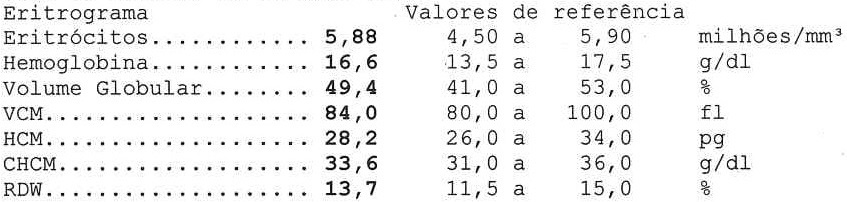
\includegraphics[width=0.80\textwidth]{img/eritrograma.jpg}
	\legend{Fonte: Elaborada pelo autor.}
	\label{fig:eritrograma}
\end{figure}
 
\subsubsection{Leucograma}
O objetivo do leucograma ao realizar a análise da parte branca do sangue, assim como no eritrograma, é analisar alguns atributos chave, porém diferente do processo anterior, essa etapa terá um foco muito maior na classificação e contagem de diferentes células brancas.

Primeiramente é feita uma contagem geral de leucócitos em mm³. Depois é realizada a contagem de forma a classificar cada tipo de leucócito presente, com neutrófilos, eosinófilos, basófilos, linfócitos, monócitos e também os granulócitos imaturos (promielócitos, mielócitos, metamielócitos). Por fim, também é calculado o número presente de plaquetas no sangue em mm³ \cite{interpretacaoHemograma, manualHematologia}.

Podemos visualizar a maneira que os índices e classificações são abordados em um hemograma real através da imagem \ref{fig:leucograma}.

\begin{figure}[!htb]
	\centering
	\caption{Exemplo de Leucograma e seus Atributos}
	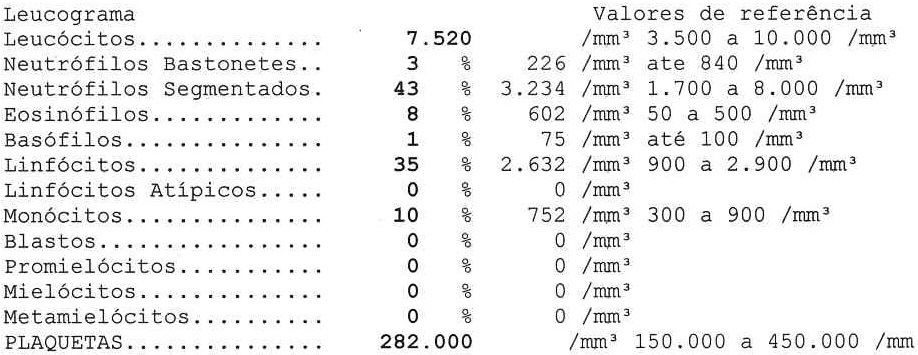
\includegraphics[width=0.80\textwidth]{img/leucograma.jpg}
	\legend{Fonte: Elaborada pelo autor.}
	\label{fig:leucograma}
\end{figure}

\section{Inteligência Artificial: Machine Learning e Deep Learning}
\label{sec:conceito2}
A abordagem de \emph{Deep Learning} que é objeto de estudo desse trabalho é uma das subáreas de \emph{Machine Learning} que por sua vez é subárea de Inteligência Artificial, portanto antes de abordar cada um desses conceitos, quais suas diferenças e aplicações, se faz necessário comentar sobre a Inteligência Artificial.

A Inteligência Artificial é uma abordagem para a resolução de problemas de diversas naturezas através de uma forma automatizada, ou seja, é uma maneira de se resolver problemas sem a necessidade de um humano ou usuário específico para esse trabalho. Essa área está muito em alta nos dias de hoje, buscando cada vez novas maneiras de automatizar a vida humana. Podemos encontrar essa abordagem em diversos segmentos da indústria e atualmente também vem crescendo o uso dentro das residências para os mais diversos usos \cite{inteligenciaArtificial}.

O intuito dessa área é buscar formas de ensinar máquinas e computadores a serem capazes de ter uma inteligência cada vez mais semelhante aos seres humanos, isso ocorre geralmente através do reconhecimento de padrões por esses dispositivos, onde eles serão ensinados a analisar dados e interpretar-los, muito semelhante ao que acontece para o aprendizado de seres humanos. Porém, diferente de nós, as máquinas geralmente precisam de um volume massivo de dados para que sejam capazes de aprender algo básico \cite{IAAprendizadoMaquina}.

\subsection{Machine Learning}

A resolução de problemas através de ferramentas da computação é bastante comum e para isso se faz uso de algoritmos programados para essa finalidade específica, porém não é em todos os problemas que podemos aplicar essa abordagem tradicional, devido ao fato de que nem sempre se sabe um caminho único de etapas a serem seguidas para resolução dos problemas. No caso, quando se sabe a entrada de dados e o resultado onde queremos chegar, mas não os meios para se chegar nesse resultado, é possível utilizar um modelo de \emph{Machine Learning} para realizar a predição. Podemos pensar que na abordagem de algoritmos tradicionais de programação possuímos os parâmetros necessários e conhecemos o método para assim chegar ao resultado, mas na aplicação de \emph{Machine Learning}, conhecemos os parâmetros e o resultado, porém o método será aprendido e apresentado pela máquina \cite{machineLearning}.

É possível fazer uma analogia entre um modelo de \emph{Machine Learning} com uma criança que está a aprender algo novo, onde todo modelo passará por três principais etapas, primeiramente o pré-processamento dos dados, depois pela fase de treinamento e por fim será realizado os devidos testes. Dessa forma, um modelo de \emph{Machine Learning} deverá ser treinado antes de realizar a predição de qualquer valor ou resultado, onde o responsável pelo treinamento deverá fornecer um grande volume de dados, assim como os resultados esperados por cada um deles. Dessa forma o modelo poderá aprender a entender e interpretar os dados de forma correta, para assim ser capaz de reproduzir esse mecanismo para prever o resultado de futuros dados \cite{machineLearningPython}.

Após o treinamento do modelo como um todo, na fase de teste, para testar e avaliar o treinamento do modelo, também é possível aplicar algumas formas e técnicas para medir o desempenho como um todo, apontando fatores interessantes como o nível de assertividade, a precisão e também o número de acertos e erros relacionados com falsos positivos e falsos negativos através de uma matriz de confusão semelhante à imagem \ref{fig:confusionMatrix} \cite{machineLearningTensorFlow}.

\begin{figure}[!htb]
	\centering
	\caption{Matriz de Confusão}
	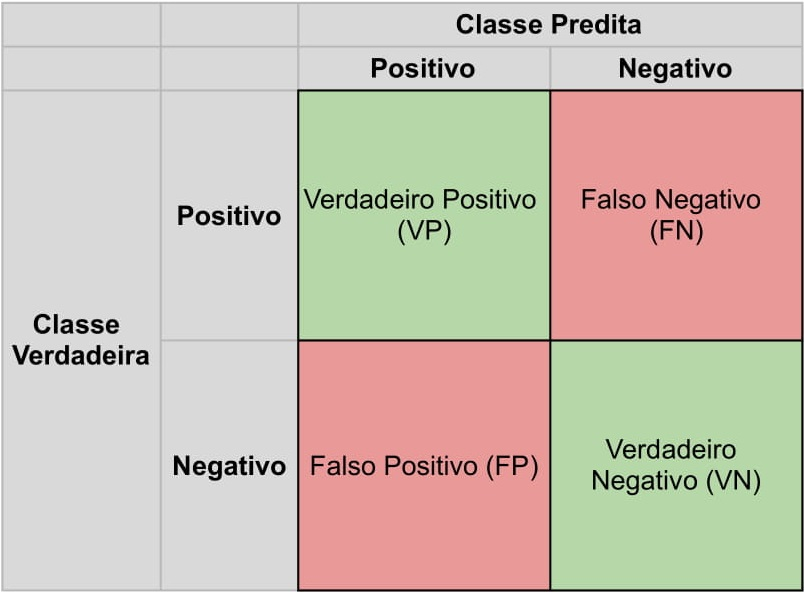
\includegraphics[width=0.50\textwidth]{img/confusionMatrix.jpg}
	\legend{Fonte: Elaborada pelo autor.}
	\label{fig:confusionMatrix}
\end{figure}

Existem várias abordagens de \emph{Machine Learning} e elas podem ser classificadas em várias categorias diferentes, porém sempre podemos dividir em duas principais abordagens mais utilizadas, sendo elas a regressão e a classificação. Os modelos de regressão serão responsáveis pela predição de valores reais, enquanto que os modelos de classificação serão responsáveis pela rotulação dos dados em determinadas classes. Além disso, também podemos classificar os algoritmos em supervisionados ou não supervisionados. No aprendizado supervisionado, sabemos o resultado correto, ou seja, onde o modelo deverá chegar a partir dos dados obtidos, porém no aprendizado não supervisionado, o modelo terá que lidar com dados não estruturados e sem um resultado claro \cite{machineLearningPython}.

\subsection{Deep Learning}
Existe alguns casos que o \emph{Machine Learning} não é suficiente para o aprendizado a partir dos dados, isso ocorre pois o aprendizado acontece através de reconhecimento de padrões com base nos dados e esses dados não podem ser utilizados de qualquer forma, devem ser preparados e adaptados para cada modelo, ou seja, a máquina não será capaz de aprender por conta própria pois sempre precisará de intervenção humana para o processamento dos dados. Logo se necessita de uma abordagem muito mais parecida com a forma de pensar dos seres humanos, como o \emph{Deep Learning} \cite{deepLearningPython, deepLearningTensorFlow}.

O \emph{Deep Learning} busca uma abordagem bastante parecida com o cérebro humano, isso acontece pois utiliza uma estrutura composta de \emph{perceptrons}, que são uma versão computadorizada de algo parecido com um neurônio humano. O \emph{perceptron} será capaz de receber inputs (os dados de entrada) e reproduzir uma saída esperada, porém ao se trabalhar com apenas um \emph{perceptron}, muitas vezes não possui o processamento necessário para se chegar a uma solução, portanto é necessário utilizar um número maior de \emph{perceptrons} conectados uns aos outros se assemelhando ainda mais ao cérebro humano. Para essa estrutura se dá o nome de rede neural artificial ou como é conhecida, \emph{Artificial Neural Network (ANN)} \cite{deepLearning, deepLearningTensorFlow}.

A figura \ref{fig:perceptron} apresenta toda a estrutura de um perceptron, onde o X representa a informação repassada, o W representa os pesos de cada informação, a letra Sigma o somatório, o F a função de ativação e por fim o Y representará a saída.

\begin{figure}[!htb]
	\centering
	\caption{Perceptron}
	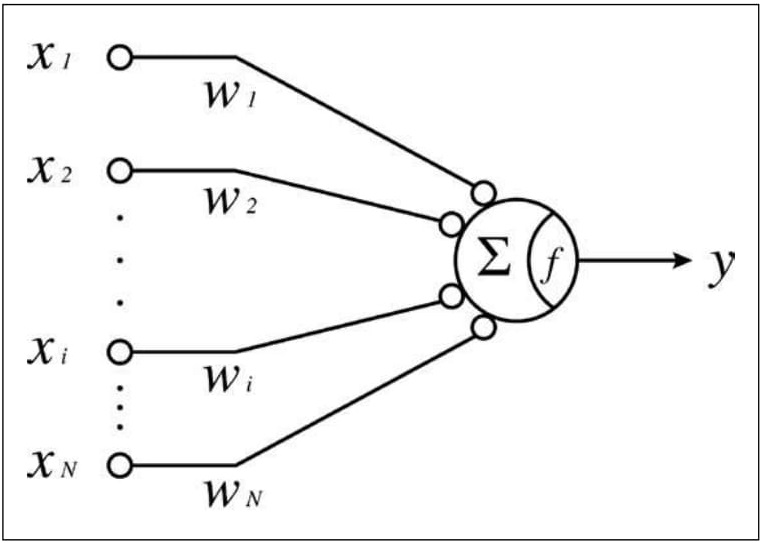
\includegraphics[width=0.50\textwidth]{img/perceptron.jpg}
	\legend{Fonte: \cite{deepLearning}}
	\label{fig:perceptron}
\end{figure}

\subsubsection{Artificial Neural Network (ANN)}
Uma \emph{Artificial Neural Network} é uma estrutura formada por diversos neurônios, conhecidos como \emph{perceptrons}, organizados de forma a imitar o processamento de um cérebro humano. Sua estrutura é definida em diversas camadas, geralmente adotando uma camada de entrada, outra de saída e camadas intermediárias chamadas de camadas ocultas que serão responsáveis pelo processamento como um todo, onde cada uma delas pode conter um número variável de \emph{perceptrons} \cite{deepLearningTensorFlow}.

\begin{figure}[!htb]
	\centering
	\caption{Artificial Neural Network}
	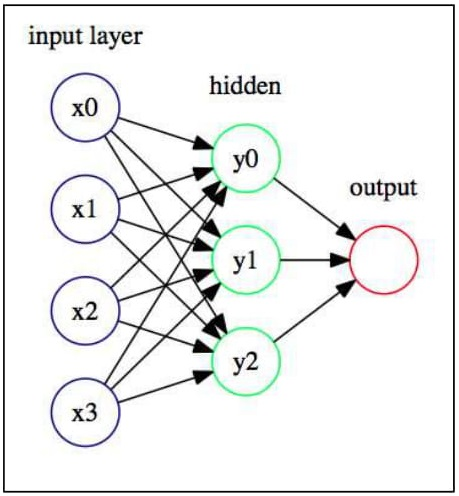
\includegraphics[width=0.40\textwidth]{img/neuralNetwork.jpg}
	\legend{Fonte: \cite{deepLearningPython}}
	\label{fig:neuralNetwork}
\end{figure}

É importante ressaltar que além das informações repassadas de um \emph{perceptron} para o outro, existe um outro fator importantíssimo para o seu funcionamento, que são os pesos adotados. Os pesos são valores definidos para cada informação recebida pelo \emph{perceptron} e podemos pensar no seu uso como um critério de prioridade entre uma informação e outra, que serão ajustados para alcançar o resultado desejado \cite{deepLearningTensorFlow}.

Dessa forma, uma ANN poderá aprender a realizar diversos tipos de tarefas, como classificação por exemplo, através do uso de um algoritmo de \emph{backpropagation} que significa propagação regressiva, responsável por gerir a taxa de aprendizado do modelo, seguindo alguns passos \cite{deepLearningTensorFlow}.

Primeiramente, o algoritmo inicializará a rede artificial com pesos aleatórios, entrando em modo de treino para realizar o aprendizado. Durante o treinamento, o algoritmo será capaz de realizar predições de resultados que serão comparados com os valores corretos, para saber se está obtendo sucesso ou não. O algoritmo de \emph{backpropagation} então irá calcular a diferença do resultado obtido com o real, e essa informação do erro será repassada para todas as camadas anteriores de forma a realizar um ajuste nos pesos e minimizar o erro \cite{deepLearningTensorFlow}.

Todo esse processo é realizado muitas vezes durante o treinamento, e só irá encerrar quando os ajustes levarem ao aumento do erro novamente, indicando que os pesos foram ajustados até o limite. Essa etapa de otimização dos pesos utilizados pela rede é muito importante de forma a ser essencial para o funcionamento da rede neural, pois através dela que é possível para o modelo aprender com os seus erros \cite{deepLearningTensorFlow}.

\subsubsection{Deep Neural Networks (DNNs)}
As \emph{Deep Neural Networks}, ou Redes Neurais Profundas, são uma arquitetura de rede neural extremamente orientada ao \emph{Deep Learning}, ou seja, embora possuam uma arquitetura semelhante às redes neurais tradicionais, são muito mais complexas em seus modelos, com um número maior de neurônios, camadas ocultas e conexões entre neurônios. Além do fato de utilizarem os princípios de aprendizagem do \emph{Machine Learning} tradicional, como o aprendizado supervisionado, como visto anteriormente \cite{deepLearningTensorFlow}.

\subsubsection{Recurrent Neural Networks (RNNs)}
As Recurrent Neural Networks, ou Redes Neurais Recorrentes, são uma arquitetura de rede neural desenvolvida para a interpretação de dados temporais em sequência, ou seja, é capaz de realizar predições de variáveis em relação ao tempo. Sua estrutura é desenvolvida para permitir conexões de feedback das informações repassadas, ou seja, possui loops que permite que as informações persistam, como se a rede fosse executada várias vezes. As RNNs são desenvolvidos para utilizar informações que possuem uma sequência fixa, como é o caso de informações que são atualizadas em decorrência do tempo \cite{deepLearningTensorFlow}.

\subsubsection{Convolutional Neural Networks (CNNs)}
As Convolutional Neural Networks, ou Redes Neurais Convolucionais, são uma arquitetura de rede neural desenvolvida especificamente para o reconhecimento de imagens, com a capacidade de interpretar imagens dividido-as em partes importantes. Essa rede trabalha inicialmente com 3 informações base, interpretando imagens como matrizes de 3 dimensões, sendo a altura, a largura e a cor \cite{deepLearningTensorFlow}.

As DNNs tradicionais funcionam bem para imagens pequenas, porém com um grande volume de dados, que nesse caso será cada pixel da imagem, o modelo teria muita dificuldade para aprender, logo nasceu a necessidade das CNNs. Para resolver esse problema, as CNNs foram desenvolvidas para usar camadas parcialmente conectadas e com grande reutilização dos pesos, dessa forma terá muito menos parâmetros a interpretar e passar adiante e consequentemente será mais rápido para treinar, terá menos risco de sobre-ajuste e requer muito menos dados de treinamento \cite{deepLearningTensorFlow}.

\begin{figure}[!htb]
	\centering
	\caption{Convolutional Neural Network}
	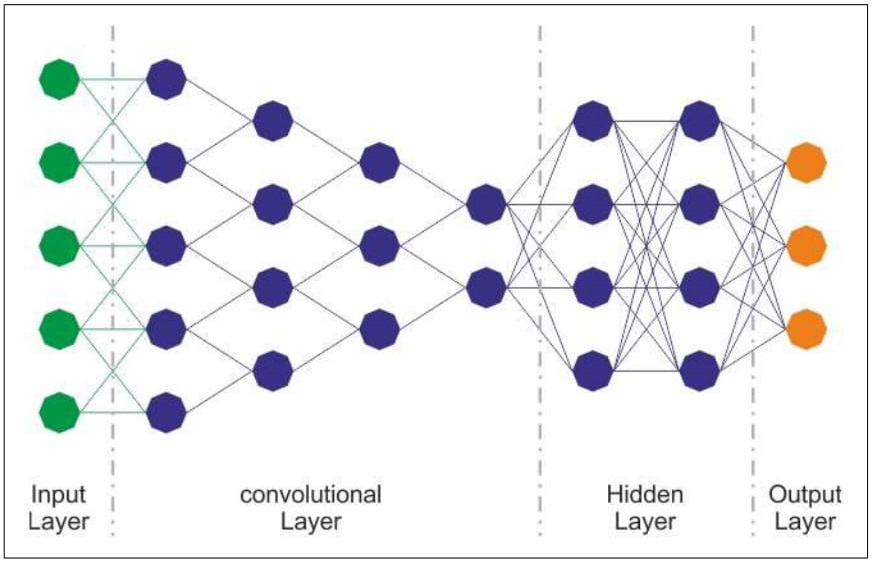
\includegraphics[width=0.60\textwidth]{img/cnn.jpg}
	\legend{Fonte: \cite{deepLearningTensorFlow}}
	\label{fig:cnn}
\end{figure}

Essa eficiência se deve também ao fato de que uma CNN quando aprender a interpretar algum recurso ou elemento específico na imagem, ela será capaz de identificar aquele elemento em qualquer lugar da imagem, diferentemente das DNNs que só aprenderia a reconhecer um recurso em um local fixo. Isso mostra a capacidade das CNNs de serem mais generalistas em comparação com as DNNs \cite{deepLearningTensorFlow}.

\subsubsection{Bibliotecas e Recursos}
Para se trabalhar com \emph{Deep Learning} e suas principais arquiteturas e recursos, existem algumas bibliotecas disponíveis no mercado de forma gratuita para esse facilitar e orientar esse trabalho. Dessa forma, pode-se encontrar o Tensorflow e o Keras, que são duas bibliotecas desenvolvidas em Python e C++, com a possibilidade de se trabalhar em conjunto bastante utilizadas pela comunidade de \emph{Deep Learning} em geral \cite{deepLearningTensorFlow}.

Através da documentação do Tensorflow, é possível encontrar informações para desenvolver uma rede neural convolucional por exemplo, onde existe toda a parte teórica e também a demonstração de um exemplo prático voltado a esse fim. Também é possível através dessa biblioteca e da sua documentação estar realizando a classificação de imagens com base em um \emph{dataset} de imagens \cite{websiteTensorFlow}.

\begin{figure}[!htb]
	\centering
	\caption{Classificação de Flores com Tensorflow}
	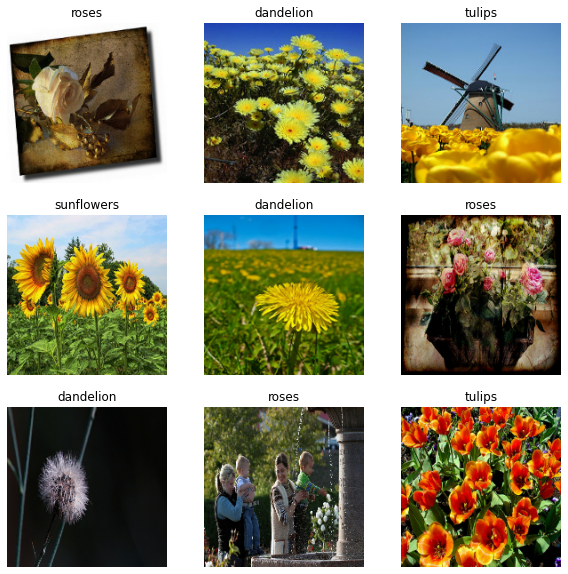
\includegraphics[width=0.60\textwidth]{img/tensorflowExample.png}
	\legend{Fonte: \cite{websiteTensorFlow}}
	\label{fig:tensorflowExample}
\end{figure}

Nesse \emph{dataset} encontra-se 3700 fotos de flores em 5 classes distintas, que irão passar pelo tratamento das imagens, divisão do \emph{dataset} em treino e teste, criação do modelo como um todo e o treinamento do modelo. Com isso é possível chegar aos resultados do treinamento comparando seu desempenho no \emph{dataset} de testes, além disso também é interessante prever novos dados externos ao \emph{dataset} para observar como o modelo se comporta e com isso tudo pode-se realizar melhorias e adaptações tanto no modelo quanto no \emph{dataset} para obter resultados ainda melhores \cite{websiteTensorFlow}.

\chapter{Estado da Arte da Área Pesquisada}
\label{chap:mapeamento}

O processo de pesquisa e seleção dos trabalhos relacionados, foi realizado com base em um mapeamento sistemático sobre as pesquisas com propostas para agilizar a identificação e interpretação de análises de sangue. Esta revisão resultou na identificação e seleção dos principais trabalhos de pesquisa no tema deste Projeto de Trabalho de Conclusão de Curso. Outro objetivo deste mapeamento sistemático foi verificar os métodos utilizados para a aplicação de \emph{Deep Learning} em imagens de sangue em placas de petri de maneira que possam ser aplicados neste projeto de forma satisfatória.

\section{Mapeamento Sistemático da Literatura}

O mapeamento sistemático da literatura é realizado com base na busca e levantamento de artigos, para isso se utiliza uma string de busca para as principais bibliotecas e repositórios de artigos. Esses artigos serão analisados e selecionados conforme a sua área de pesquisa e a sua temática, para inclusão nesse estudo. Para isso, se é utilizado uma ferramenta para automatização dessa tarefa, que é o Parsifal\footnote[1]{https://parsif.al/}, de modo a definir a string de busca, salvar os artigos necessários e realizar a seleção.

As questões de pesquisas levantadas para isso foram, ``Como os algoritmos de \emph{Deep Learning} podem ser utilizados para a interpretação de exames?'' e ``Como realizar o tratamento de imagens para reconhecimento por modelos de \emph{Deep Learning}?''. A partir dessas questões se foram extraídas palavras e termos para o direcionamento da pesquisa. Podemos visualizar estas palavras com seus sinônimos na Tabela 1.

\begin{table}[!htb]
	\centering
	\caption{Palavras-Chave e Sinônimos}
	\label{tbl:palavrasChave}
	\begin{tabular}{|c|c|}
		\hline
		\textbf{Palavra-Chave} & \textbf{Sinônimos}                                        \\ \hline
		Blood Analysis         & Blood Sample                                               \\ \hline
		Classification         & Interpretation, Recognition                                \\ \hline
		Deep Learning          & Artificial Intelligence, Computer Vision, Machine Learning \\ \hline
	\end{tabular}
	\vspace{6pt}
	\legend{Fonte: Elaborada pelo autor.}
\end{table}

Na Tabela 2, é listado as bases de dados onde os artigos foram coletados, a quantidade de cada um de les e a string de busca utilizada na seleção. A mesma string de busca foi utilizado nas três bases de dados, e os artigos encontrados foram dos últimos 5 anos.

\begin{table}[!htb]
	\centering
	\caption{Bases de Dados e Número de Artigos Selecionados}
	\label{tbl:basesDeDados}
	\begin{tabular}{|c|c|c|}
		\hline
		\textbf{Base de Dados}                & \textbf{Artigos}     & \textbf{String de Busca}                                                                                     \\ \hline
		\multirow{2}{*}{ACM Digital Library}  & \multirow{2}{*}{37}  & \multirow{6}{*}{\begin{tabular}[c]{@{}c@{}}(``classification'' OR ``interpretation'' OR ``recognition'') AND \\  (``deep learning'' OR ``artificial intelligence'' \\ OR ``computer vision'' OR ``machine learning'') AND\\  (``blood analysis'' OR ``blood sample'')\end{tabular}} \\
		                                      &                      &                                                                                                              \\ \cline{1-2}
		\multirow{2}{*}{IEEE Digital Library} & \multirow{2}{*}{13}  &                                                                                                              \\
		                                      &                      &                                                                                                              \\ \cline{1-2}
		\multirow{2}{*}{Scopus}               & \multirow{2}{*}{114} &                                                                                                              \\
		                                      &                      &                                                                                                              \\ \hline
	\end{tabular}
	\vspace{6pt}
	\legend{Fonte: Elaborada pelo autor.}
\end{table}

\subsection{Critérios de Exclusão}

Os artigos coletados na pesquisa através da string de busca, passaram por critérios de exclusão por não se adequarem a esta pesquisa, esses critérios podem ser observados na Tabela 3. 

\begin{table}[!htb]
	\centering
	\caption{Critérios de Exclusão}
	\label{tbl:exclusao}
	\begin{tabular}{|c|c|}
		\hline
		\textbf{Critério de Exclusão}                    & \textbf{Nº de Artigos Recusados} \\ \hline
		O estudo não faz parte da área de pesquisa       & 101                               \\ \hline
		O estudo apresenta resultados fora da computação & 29                                \\ \hline
		O estudo não é um estudo primário               & 6                                 \\ \hline
		O estudo é duplicado                              & 16                                \\ \hline
	\end{tabular}
	\vspace{6pt}
	\legend{Fonte: Elaborada pelo autor.}
\end{table}

A seleção inciou com 164 artigos no total das três bases de dados buscadas. Com a aplicação dos critérios de exclusão, observa-se um resultante de apenas 14 artigos. Isso ocorreu pois 101 artigos foram eliminados no critério ``O estudo não faz parte da área de pesquisa'', que significa que esses artigos tinham alguma relação, porém eram voltados a outras áreas. Outros 29 artigos foram eliminados no critério ``O estudo apresenta resultados fora da computação'', que significa que eram da área de pesquisa, porém com resultados e métodos sem conexão com a computação. Foram também encontrados 6 artigos, que entraram no critério ``O estudo não é um estudo primário'', o que indica que o artigo pode ser uma revisão sistemática da literatura ou semelhante. Por fim, foram eliminados outros 16 artigos por serem duplicados.

\subsection{Critérios de Inclusão}

Os seguintes critérios de inclusão foram definidos:
\begin{itemize}
	\item Nova tecnologia para análise de sangue;
	\item Processo, método ou técnica para contagem de células sanguíneas;
	\item Sistema para elaboração de hemogramas utilizando Deep Learning;
\end{itemize}

Na tabela 4, podemos encontrar todos os 14 artigos selecionados com base nos critérios de inclusão, todos eles se enquadram em pelo menos um deles.

\begin{table}[!htb]
	\centering
	\caption{Artigos Selecionados}
	\label{tbl:mapeamento}
	\begin{tabular}{|c|l|l|}
		\hline
		\textbf{ID} & \multicolumn{1}{c|}{\textbf{Título do Artigo}}                      \\ \hline
		A1  & \begin{tabular}[c]{@{}l@{}}Analyzing microscopic images of           \\ peripheral blood smear \\ using deep learning\end{tabular} & \begin{tabular}[c]{@{}l@{}}Mundhra, D. and Cheluvaraju, B. \\ and Rampure, J. and Rai Dastidar, T.\end{tabular} \\ \hline
		A2  & \begin{tabular}[c]{@{}l@{}}Automatic detection and classification    \\ of leukocytes using \\ convolutional neural networks\end{tabular} & \begin{tabular}[c]{@{}l@{}}Zhao, J. and Zhang, M. \\ and Zhou, Z. and Chu, J. and Cao, F.\end{tabular} \\ \hline
		A3  & \begin{tabular}[c]{@{}l@{}}Automatic white blood cell classification \\ using pre-trained deep learning models: \\ ResNet and Inception\end{tabular} & \begin{tabular}[c]{@{}l@{}}Habibzadeh, M. and Jannesari, M. \\ and Rezaei, Z. and Baharvand, H. \\ and Totonchi, M.\end{tabular} \\ \hline
		A4  & \begin{tabular}[c]{@{}l@{}}Classification of Human White             \\ Blood Cells Using Machine Learning \\ for Stain-Free Imaging \\ Flow Cytometry\end{tabular} & \begin{tabular}[c]{@{}l@{}}Lippeveld, M. and Knill, C. and \\ Ladlow, E. and \\ Fuller, A. and Michaelis, L.J. and \\ Saeys, Y. and Filby, A. and Peralta, D.\end{tabular} \\ \hline
		A5  & \begin{tabular}[c]{@{}l@{}}Blood cell classification using the hough \\ transform and \\ convolutional neural networks\end{tabular} & \begin{tabular}[c]{@{}l@{}}Molina-Cabello, M.A. and López-Rubio, E. \\ and Luque-Baena, R.M. and \\ Rodríguez-Espinosa, M.J. and \\ Thurnhofer-Hemsi, K.\end{tabular} \\ \hline
		A6  & \begin{tabular}[c]{@{}l@{}}White Blood Cells Image Classification    \\ Using Deep Learning with \\ Canonical Correlation Analysis\end{tabular} & Patil, A.M. and Patil, M.D. and Birajdar, G.K. \\ \hline
		A7  & \begin{tabular}[c]{@{}l@{}}Image processing and machine learning     \\ in the morphological analysis \\ of blood cells\end{tabular} & \begin{tabular}[c]{@{}l@{}}Rodellar, J. and Alférez, S. and Acevedo, A. \\ and Molina, A. and Merino, A.\end{tabular} \\ \hline
		A8  & \begin{tabular}[c]{@{}l@{}}Improving blood cells classification in   \\ peripheral blood smears using \\ enhanced incremental training\end{tabular} & Al-qudah, R. and Suen, C.Y. \\ \hline
		A9  & \begin{tabular}[c]{@{}l@{}}Corruption-Robust Enhancement of          \\ Deep Neural Networks\\ for Classification of Peripheral \\ Blood Smear Images\end{tabular} & \begin{tabular}[c]{@{}l@{}}Zhang, S. and Ni, Q. and Li, B. and \\ Jiang, S. and \\ Cai, W. and Chen, H. and Luo, L.\end{tabular} \\ \hline
		A10 & \begin{tabular}[c]{@{}l@{}}Convolutional neural network and decision \\ support in medical imaging:\\ Case study of the recognition of \\ blood cell subtypes\end{tabular} & Diouf, D. and Seck, D. and Diop, M. and Ba, A. \\ \hline
		A11 & \begin{tabular}[c]{@{}l@{}}Combining Convolutional Neural Network    \\ With Recursive Neural Network \\ for Blood Cell Image Classification\end{tabular} & \begin{tabular}[c]{@{}l@{}}Liang, G. and Hong, H. and Xie, W. and\\ Zheng, L.\end{tabular} \\ \hline
		A12 & \begin{tabular}[c]{@{}l@{}}Blood diseases detection using            \\ classical machine learning algorithms\end{tabular} & Alsheref, F.K. and Gomaa, W.H. \\ \hline
	\end{tabular}
	\vspace{6pt}
	\legend{Fonte: Elaborada pelo autor.}
\end{table}

Todos os artigos selecionados estão relacionados à maneiras e recursos para auxiliar na interpretação de exames de sangue utilizando conceitos de \emph{Deep Learning} e \emph{Machine Learning}.

\section{Análise dos trabalhos selecionados}

Por fim, com os artigos selecionados e classificados, é necessário realizar a extração dos dados desses trabalhos, sendo essa a última etapa desse mapeamento sistemático da literatura. É possível perceber que os algoritmos e abordagens mais utilizados são técnicas de \emph{Deep Learning}, como por exemplo, o uso de \emph{Convolutional Neural Network (CNN)} (A1, A2, A3, A4, A5, A6, A8, A9, A10, A11) e de \emph{Recurrent Neural Network (RNN)} (A6, A11), que são abordagens de redes neurais para a classificação das células sanguíneas.

Outros trabalhos utilizam de algoritmos de \emph{Machine Learning} tradicionais para a classificação, como por exemplo, ocorre com o uso de \emph{Random Forest} ou \emph{Decision Trees}  (A2, A4, A7), que são estruturas de árvores de decisão. Também se encontra estudos fazendo uso de \emph{Support Vector Machine (SVM)} (A7) que utilizam vetores de suporte e por fim \emph{K-Means e K-Nearest Neighbors (KNN)} (A12), que faz a classificação levando em conta os vizinhos mais próximos.

\chapter{Procedimentos Metodológicos}
\label{chap:metodologia}

% Quanto à natureza = Aplicada
% Quanto ao estilo de pesquisa = Empírica
% Quanto aos objetivos = Exploratória
% Quanto aos procedimentos metodológicos = Bibliográfica

O projeto iniciou com uma pesquisa exploratória da bibliografia para delimitar o escopo e compreender melhor os aspectos que estão sendo aplicados para o domínio de problema abordado por este trabalho. Essa pesquisa exploratória permitiu elaborar um mapeamento sistemático da literatura e também desenvolver uma fundamentação teórica a partir disso.

Em sequência, o que será buscado por este trabalho é a coleta dos datasets selecionados para a pesquisa, assim como realizar os devidos tratamentos e análise aprofundada desse material, de forma a preparar uma base de dados sólida e confiável para o prosseguimento dos trabalhos. Esses datasets estão disponíveis na internet de forma aberta e gratuita.

Com o dataset devidamente ajustado, pode-se iniciar a preparação do modelo de \emph{Deep Learning}. De forma, a definir as camadas que o modelo deverá ter, com base nas imagens contidas no dataset. Com o modelo desenvolvido, iniciará a fase de treinamento e depois de teste do modelo em si, onde o dataset será divido em treino e teste, geralmente adotando uma proporção de 70\% de dados para o treino e 30\% de dados para o teste.

Os modelos de \emph{Deep Learning} após esse processo podem ser avaliados em relação ao seu desempenho, verificando métricas importantes do aprendizado como acurácia, revocação e precisão. Além dessa análise, se pode também preparar uma matriz de confusão para uma melhor visualização do desempenho do modelo em si. Dependendo do resultado recebido, o modelo poderá passar por modificações e melhorias para um resultado mais assertivo e consequentemente mais confiável.

Por fim, ao atingir o objetivo desejado, os dados dos resultados e da performance do modelo serão registrados e descritos no trabalho de conclusão de curso final. Além disso será feita uma comparação dessa solução com as demais encontradas por outros modelos documentados na literatura.

\section{Recursos}
\label{chap:recursos}

Os recursos que serão utilizados para o desenvolvimento deste projeto serão um computador próprio, todos os recursos disponibilizados pelo IFSC, como a sua biblioteca física e virtual, também serão consultados os artigos encontrados nos repositórios online disponíveis. Além disso serão consultados datasets e conjuntos de dados disponíveis de forma online para este fim. A impressão do trabalho será terceirizada.

\chapter{Cronograma}
\label{chap:cronograma}

A Tabela \ref{tbl:cronograma} apresenta o cronograma de atividades propostas para o desenvolvimento deste projeto de trabalho de conclusão de curso, de forma a viabilizar a produção automática de hemogramas utilizando modelos de \emph{Deep Learning}.

\begin{table}[!htb]
	\centering
	\caption{Cronograma das atividades previstas.}
	\label{tbl:cronograma}
\begin{tabular}{|l|c|c|c|c|c|c|c|c|c|c|}
\hline 
\multicolumn{1}{|c|}{\textbf{Etapa}} & \multicolumn{10}{c|}{\textbf{Meses}} \\ \hline
 & Fev & Mar & Abr & Mai & Jun & Ago & Set & Out & Nov & Dez \\ \hline
Fundamentação Teórica & X & X &  &  &  &  &  &  &  &  \\ \hline
\begin{tabular}[c]{@{}l@{}}Mapeamento Sistemático\\ da Literatura\end{tabular} &  &  & X & X &  &  &  &  &  &  \\ \hline
\begin{tabular}[c]{@{}l@{}}Escrita do Projeto de\\  TCC e Defesa\end{tabular} &  &  & X & X & X &  &  &  &  &  \\ \hline
\begin{tabular}[c]{@{}l@{}}Análise e Tratamento\\ dos Dados\end{tabular} &  &  &  &  &  & X &  &  &  &  \\ \hline
\begin{tabular}[c]{@{}l@{}}Treinamento dos Modelos\\ de Deep Learning\end{tabular} &  &  &  &  &  &  & X &  &  &  \\ \hline
\begin{tabular}[c]{@{}l@{}}Análise dos Resultados\\ dos Modelos\end{tabular} &  &  &  &  &  &  & X & X &  &  \\ \hline
\begin{tabular}[c]{@{}l@{}}Verificação de Aceitação\\ dos Resultados\end{tabular} &  &  &  &  &  &  &  & X &  &  \\ \hline
\begin{tabular}[c]{@{}l@{}}Comparação dos Resultados\\ com a Literatura\end{tabular} &  &  &  &  &  &  &  & X & X &  \\ \hline
Exposição dos Resultados &  &  &  &  &  &  &  &  & X &  \\ \hline
Escrita do TCC &  &  &  &  &  &  &  &  & X & X \\ \hline
Defesa do TCC &  &  &  &  &  &  &  &  &  & X \\ \hline
\end{tabular}
	\vspace{6pt}
	\legend{Fonte: Elaborada pelo autor.}
\end{table}

As atividades propostas neste cronograma podem sofrer leves alterações no decorrer do seu desenvolvimento de acordo com a necessidade.